\documentclass[11pt,a4paper]{article}
\usepackage{graphicx}
\usepackage{mathptmx}
\usepackage[T1]{fontenc}
\usepackage{epsfig}
\usepackage{amsmath}
\usepackage{amsfonts}
\usepackage{amssymb}
\usepackage[ngerman]{babel}
\usepackage[utf8]{inputenc}
\usepackage{multirow}
\usepackage{float}
\usepackage[height=23cm,width=14.3cm]{geometry}

\begin{document}

\title{Hochleistungsrechnen - Übungsblatt 11}
\author{Joscha Fregin, Tim Kilian, Stefan Knispel}
\maketitle



\section{Verwendung von 3 Prozessen und 2 Knoten}



\subsection{Jacobi-Verfahren}


\subsubsection{Startphase des Programms}
Hier ist schön zu sehen, dass der Prozess 1 nach der Initialisierung seine Berechnung startet. Der Prozess 2 wartet nach seiner Initialisierung auf den Prozess 1 und fängt nach dem Empfangen auch an zu rechnen. Der dritte Prozess wartet auf den zweiten und rechnet nach Empfang ebenfalls los.
\begin{figure}[htbp] %  figure placement: here, top, bottom, or page
   \centering
   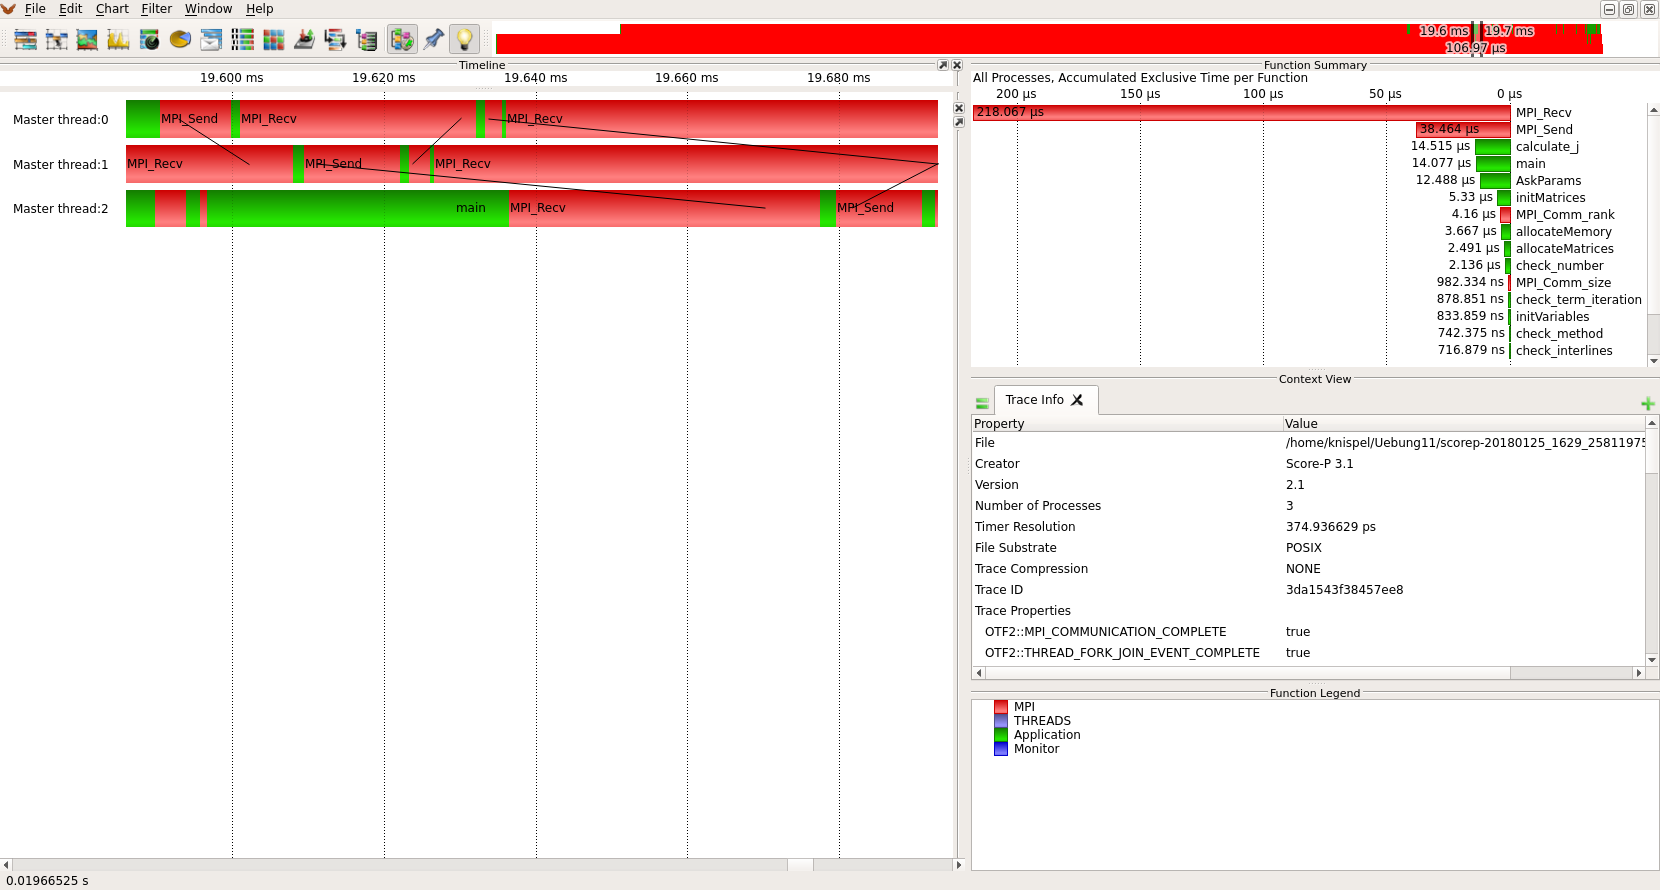
\includegraphics[width=1\textwidth]{Jacobi_1.png} 
   \caption{Jacobi-Verfahren mit 3 Prozessoren und 2 Knoten : Startphase}
   \label{Jacobi_1}
\end{figure}

\subsubsection{Phase der Synchronisation}
Hier ist schön zu sehen, dass die einzelnen Prozesse ihre Berechnung kurz unterbrechen, um die erste schon berechnete Zeile an den darüberliegenden Prozess zu schicken. Danach rechnen sie weiter und schicken am Ende ihre letzte Zeile an den unteren Prozess.

\begin{figure}[htbp] %  figure placement: here, top, bottom, or page
   \centering
   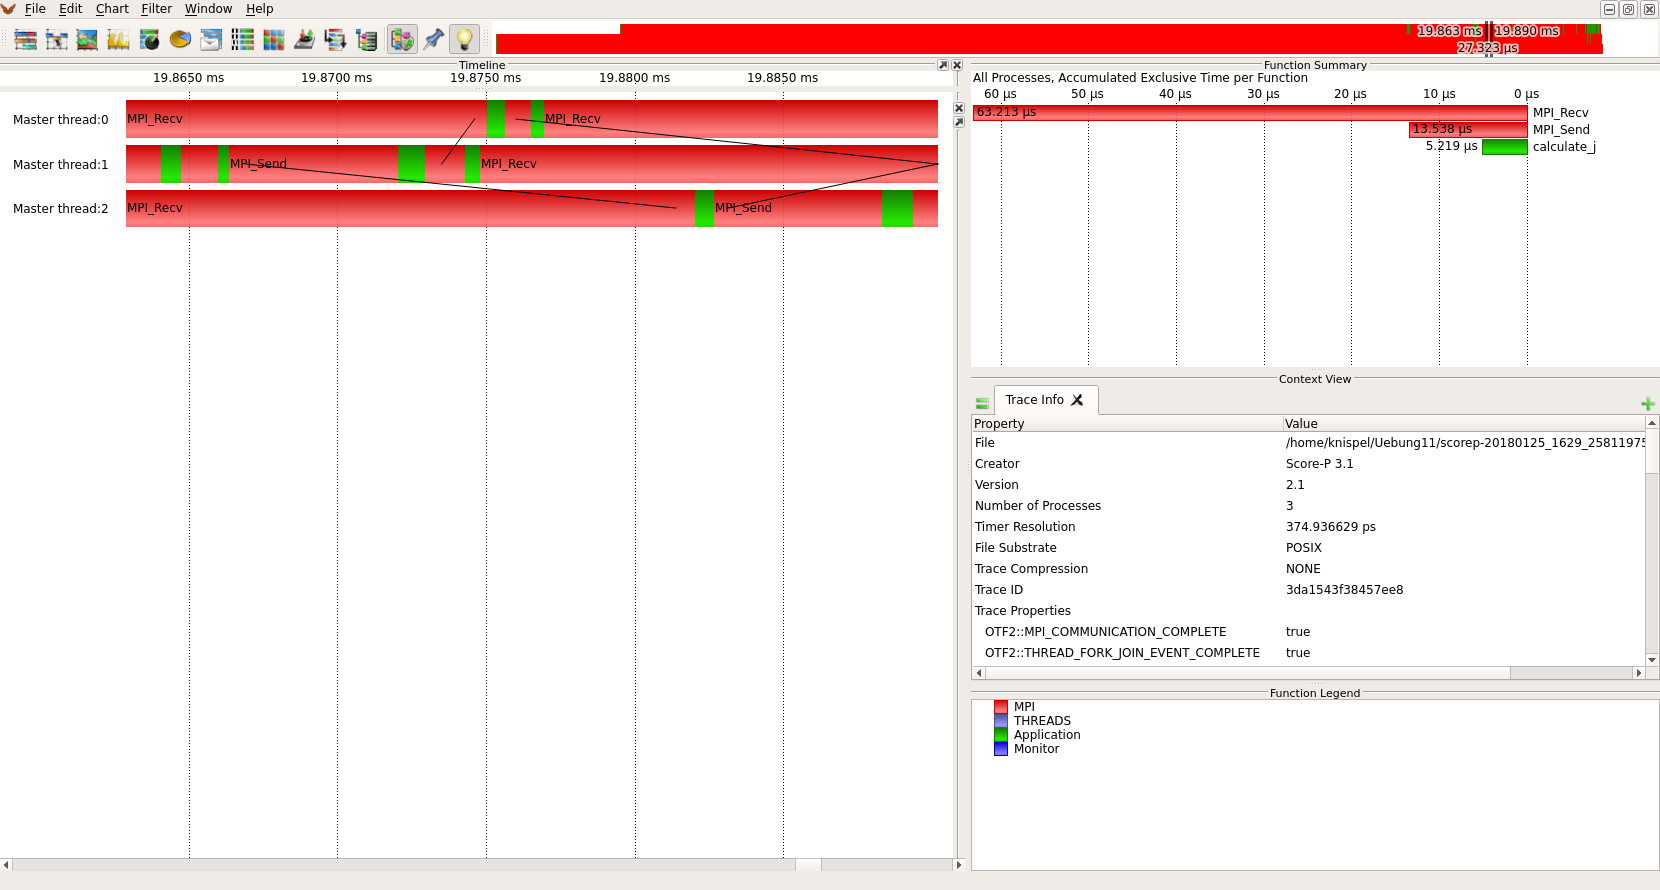
\includegraphics[width=1\textwidth]{Jacobi_2.png} 
   \caption{Jacobi-Verfahren mit 3 Prozessoren und 2 Knoten : Phase der Synchronisation}
   \label{Jacobi_2}
\end{figure}

\subsubsection{Phase des Einsammelns}
Bei allen drei Prozessen ist die Phase des Allreduce zu sehen. Nachdem der erste Prozess fertig ist, sammelt er dann die Informationen der anderen Prozesse ein. Auch ist zu erkennen, dass die anderen Prozesse auf das Verteilen der Informationen des nullten Prozesses warten und danach erfolgt noch eine kleine weitere Berechnung auf jedem Prozess.

\begin{figure}[htbp] %  figure placement: here, top, bottom, or page
   \centering
   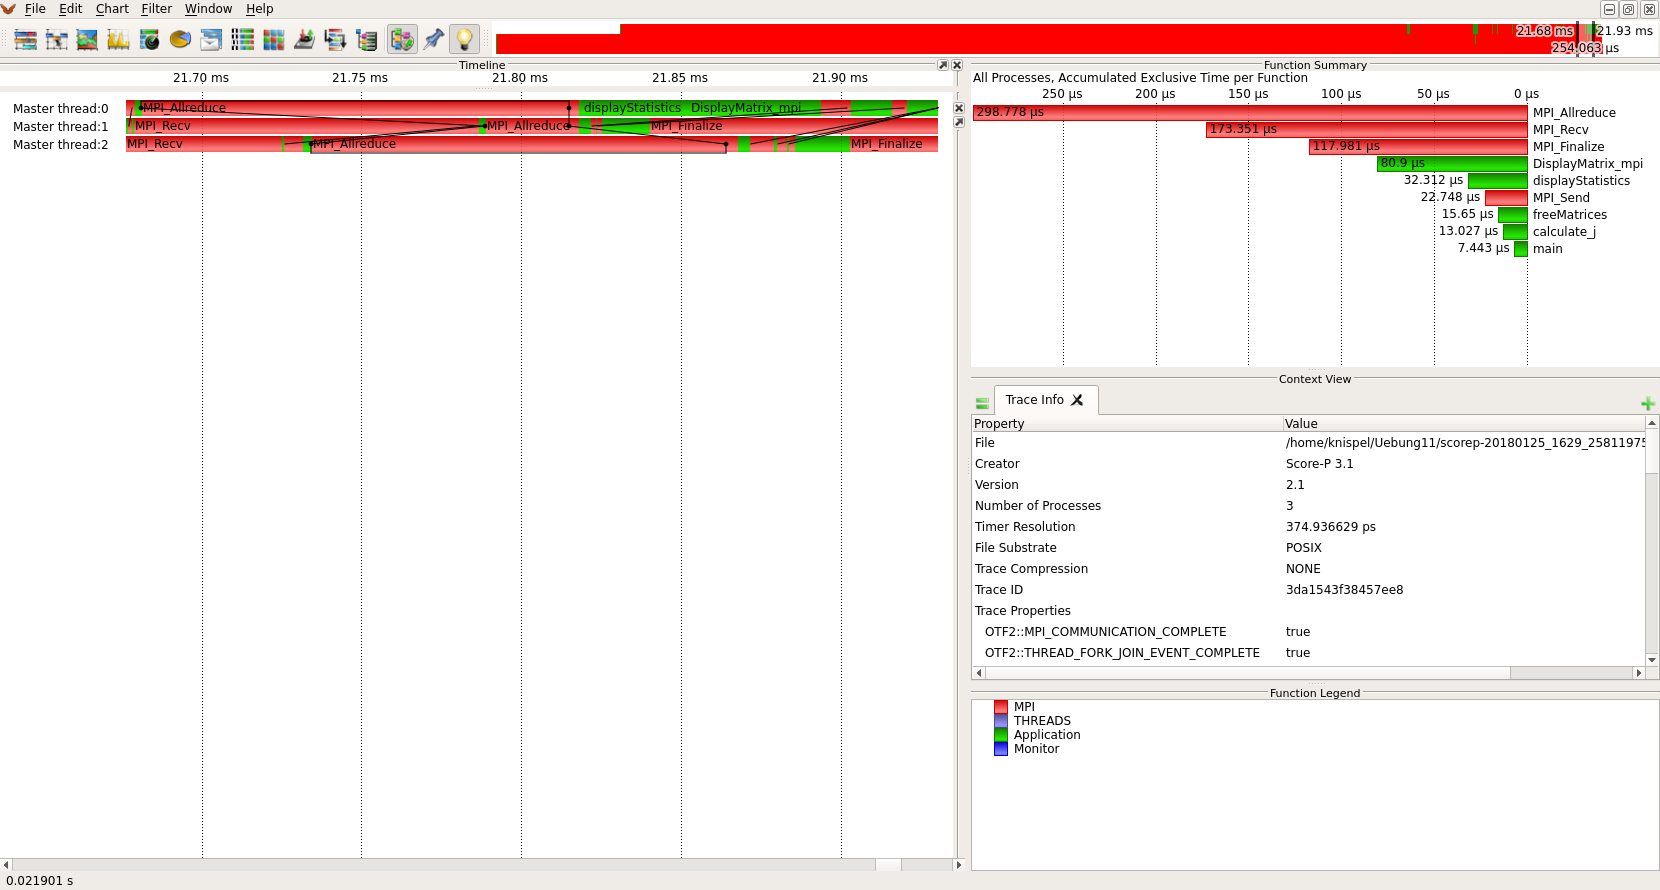
\includegraphics[width=1\textwidth]{Jacobi_3.png} 
   \caption{Jacobi-Verfahren mit 3 Prozessoren und 2 Knoten : Phase des Einsammelns}
   \label{Jacobi_3}
\end{figure}


\subsection{Gauß-Seidel-Verfahren}


\subsubsection{Startphase des Programms}
Die Startphase ist so wie bei Jacobi. Nach der Initialisierung warten die Prozesse auf den Prozess darüber.
\begin{figure}[htbp] %  figure placement: here, top, bottom, or page
   \centering
   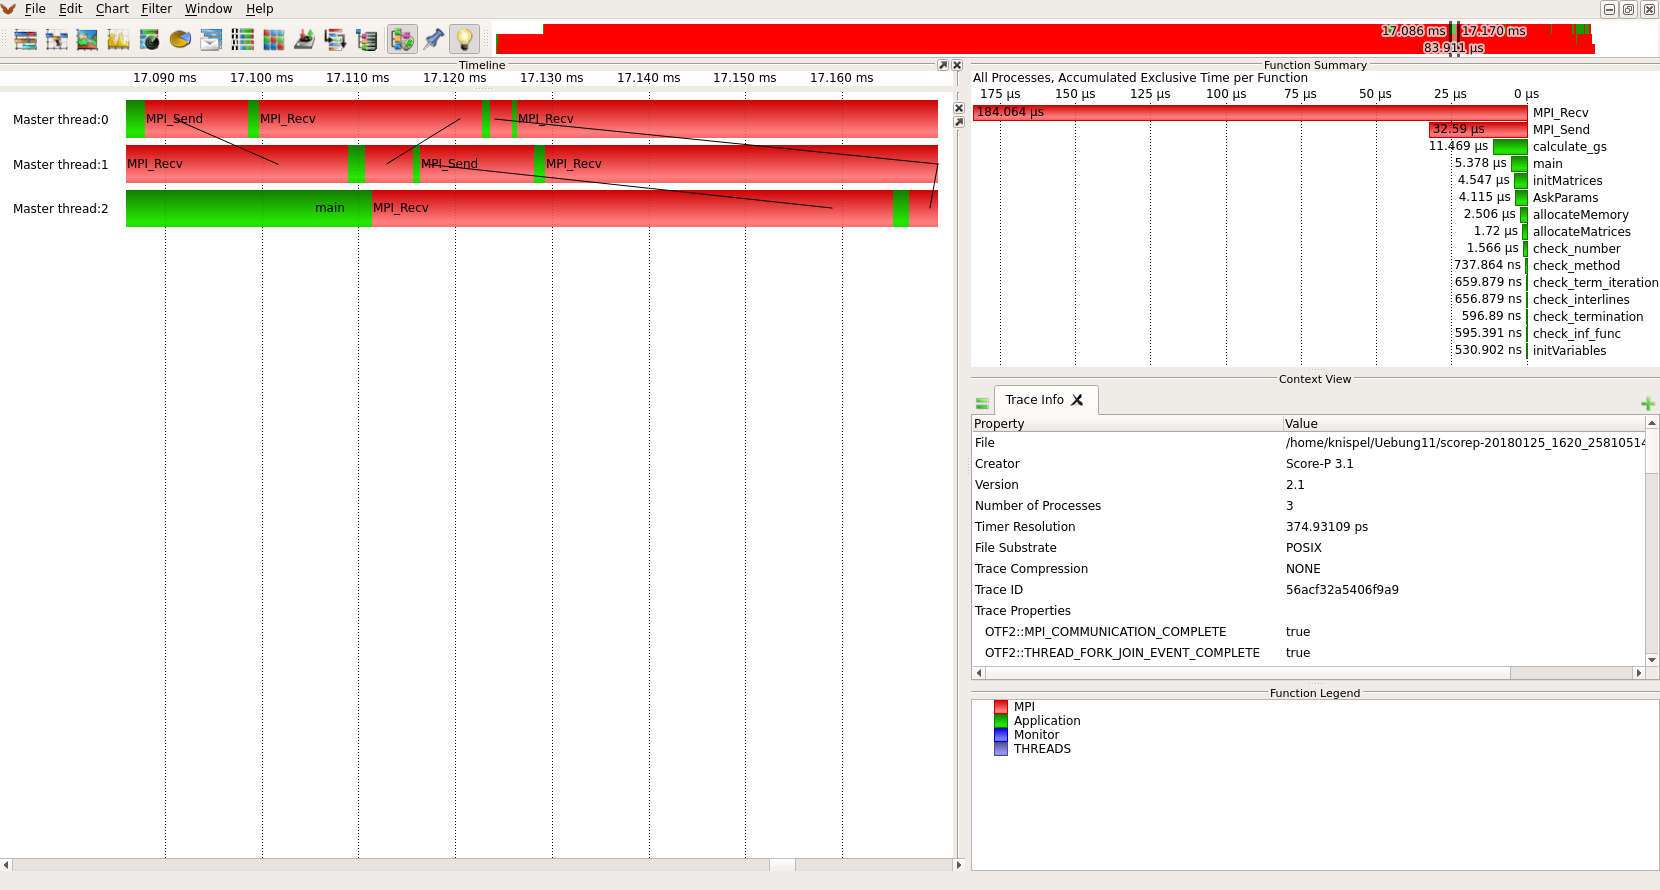
\includegraphics[width=1\textwidth]{Seidel_1.png} 
   \caption{Gauß-Seidel-Verfahren mit 3 Prozessoren und 2 Knoten : Startphase}
   \label{Seidel_1}
\end{figure}

\subsubsection{Phase der Synchronisation}
Auch hier ist das gleiche Spiel wie bei Jacobi zu sehen, nur dass die aktuelle Iteration unterschiedlich ist.
\begin{figure}[htbp] %  figure placement: here, top, bottom, or page
   \centering
   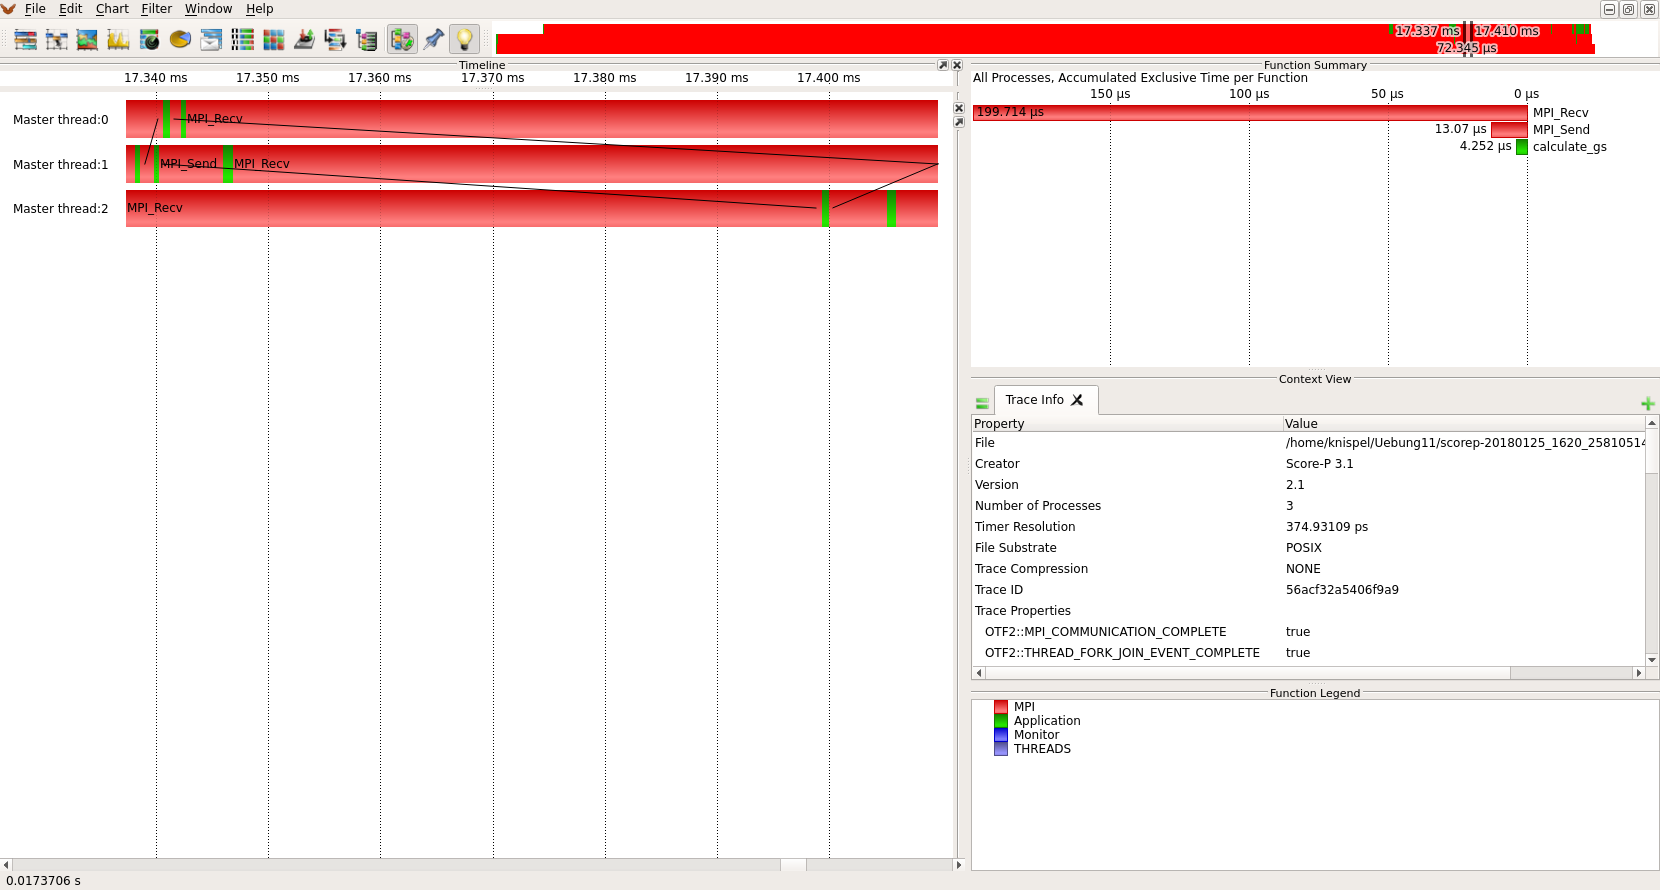
\includegraphics[width=1\textwidth]{Seidel_2.png} 
   \caption{Gauß-Seidel-Verfahren mit 3 Prozessoren und 2 Knoten : Phase der Synchronisation}
   \label{Seidel_2}
\end{figure}

\subsubsection{Phase des Einsammelns}
Bei dem Allreduce wird wieder durch den nullten Prozess eingesammelt ( kann man erkennen) und er verteilt danach die Informationen an die folgenden Prozesse. Da die anderen Prozesse dadurch ihre Information erhalten, wie viele Iterationen sie noch rechnen müssen, folgt darauf wieder ein Block von Berechnungen. Danach beenden auch hier alle Prozesse und Prozess null leitet die Funktion display-matrix ein.
\begin{figure}[htbp] %  figure placement: here, top, bottom, or page
   \centering
   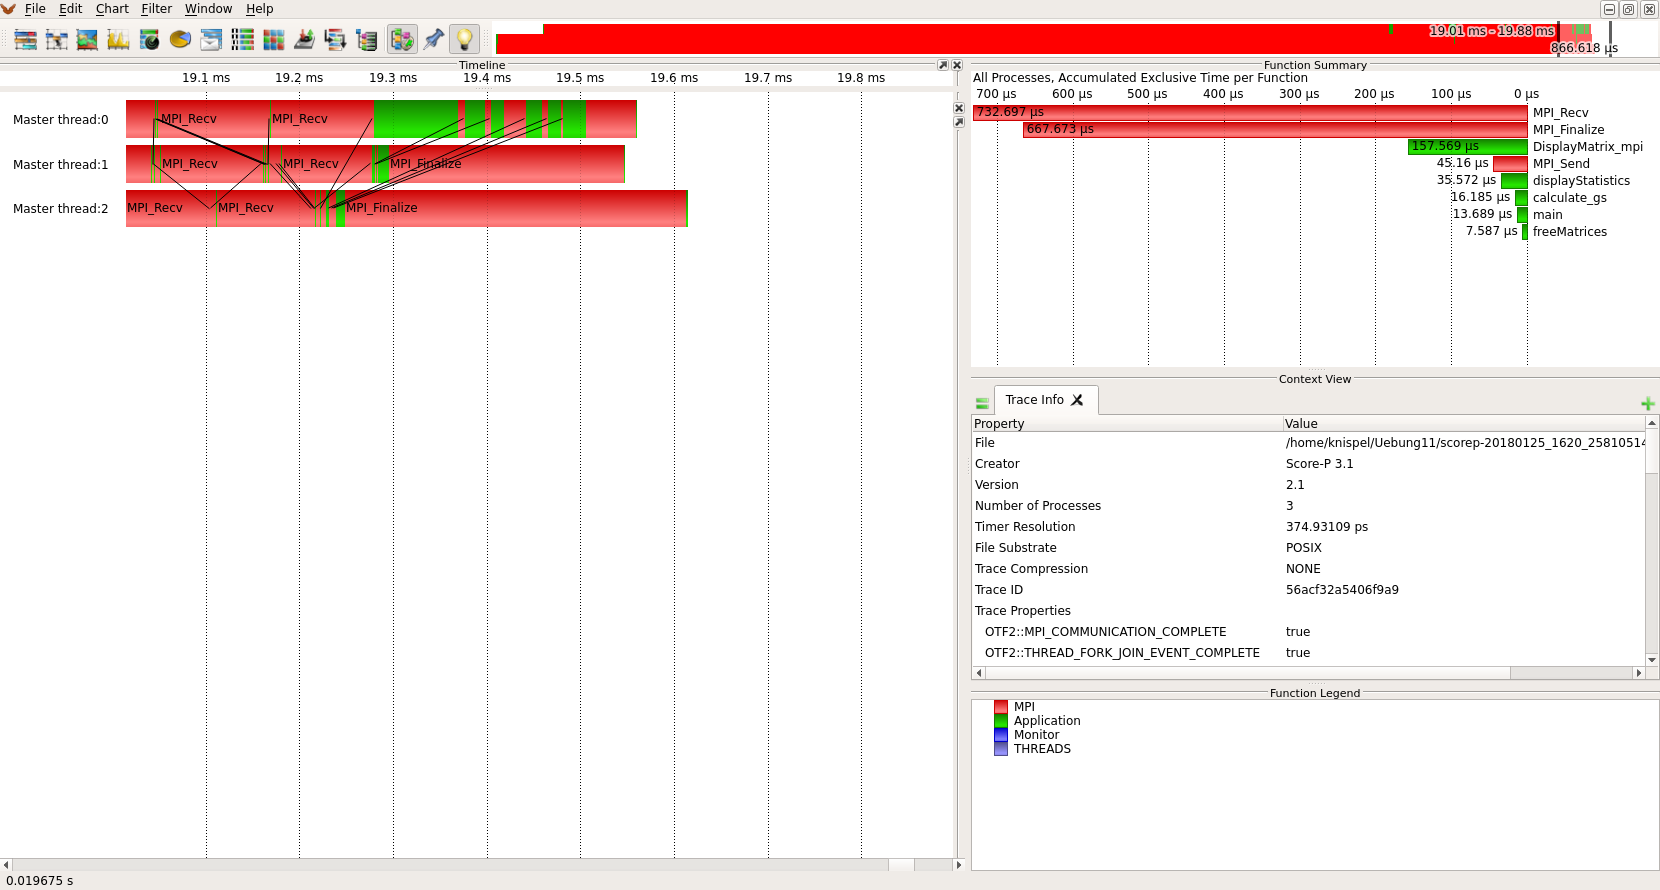
\includegraphics[width=1\textwidth]{Seidel_3.png} 
   \caption{Gauß-Seidel-Verfahren mit 3 Prozessoren und 2 Knoten : Phase des Einsammelns}
   \label{Seidel_3}
\end{figure}




\section{Verwendung von 5 Prozessen und 4 Knoten}

Bei der Verwendung von 5 Prozessen und 4 Knoten kann man die gleiche Vorgehensweise erkennen wie bei den Einstellungen darüber. Daher folgt hier keine weitere Erklärung dazu.

\subsection{Jacobi-Verfahren}


\subsubsection{Startphase des Programms}

\begin{figure}[htbp] %  figure placement: here, top, bottom, or page
   \centering
   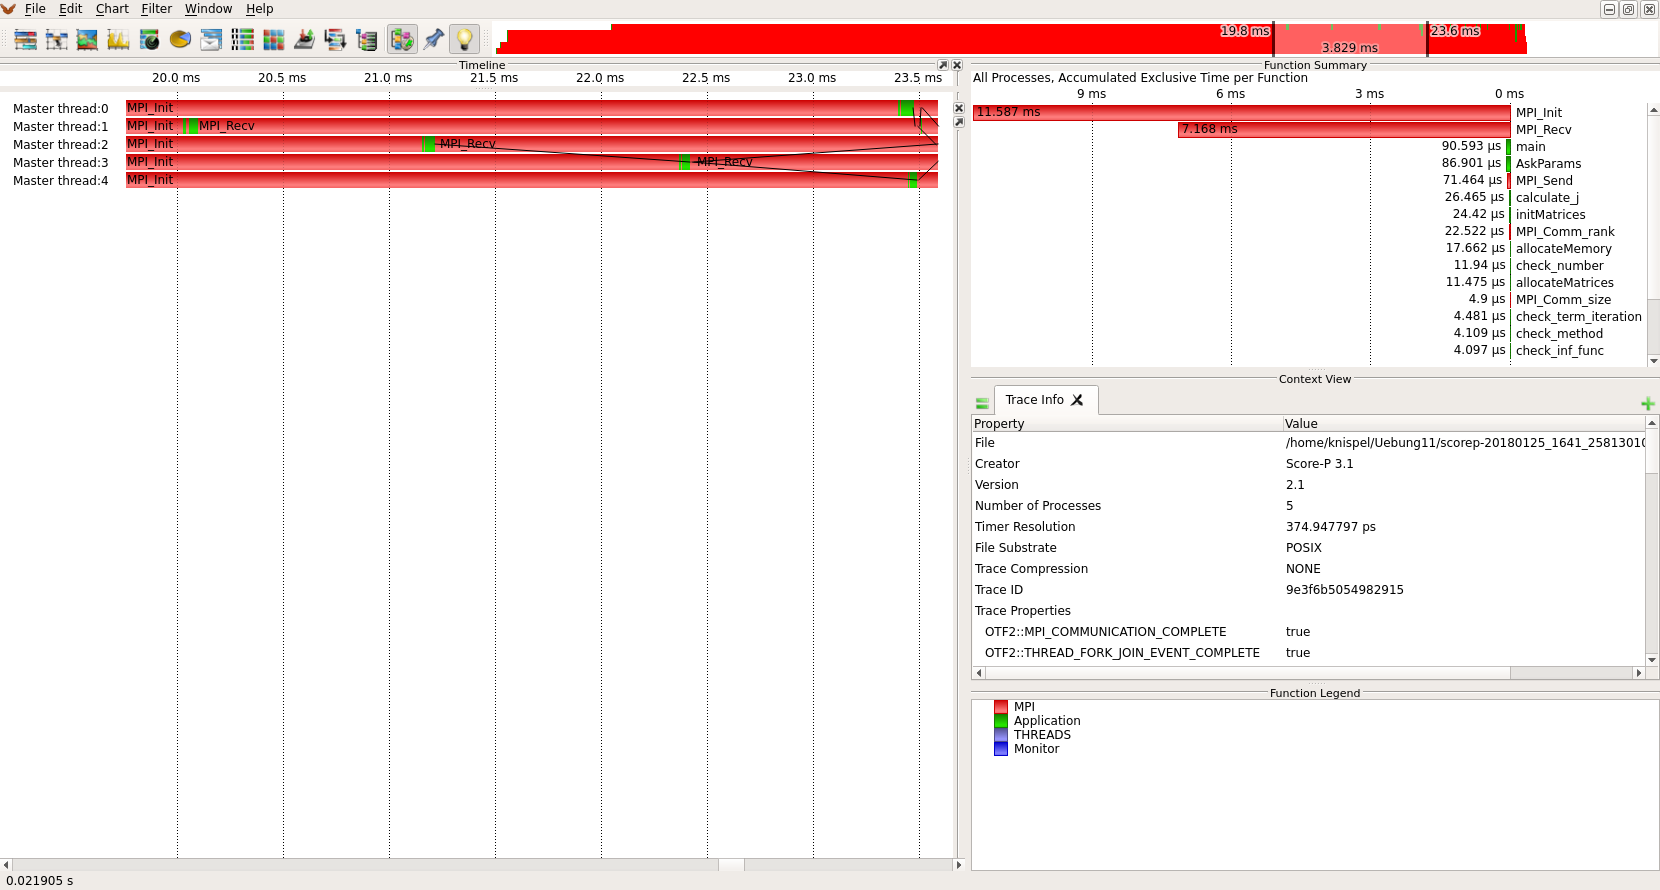
\includegraphics[width=1\textwidth]{Jacobi_1_4nodes.png} 
   \caption{Jacobi-Verfahren mit 5 Prozessoren und 4 Knoten : Startphase}
   \label{Jacobi_1_4nodes}
\end{figure}

\subsubsection{Phase der Synchronisation}

\begin{figure}[htbp] %  figure placement: here, top, bottom, or page
   \centering
   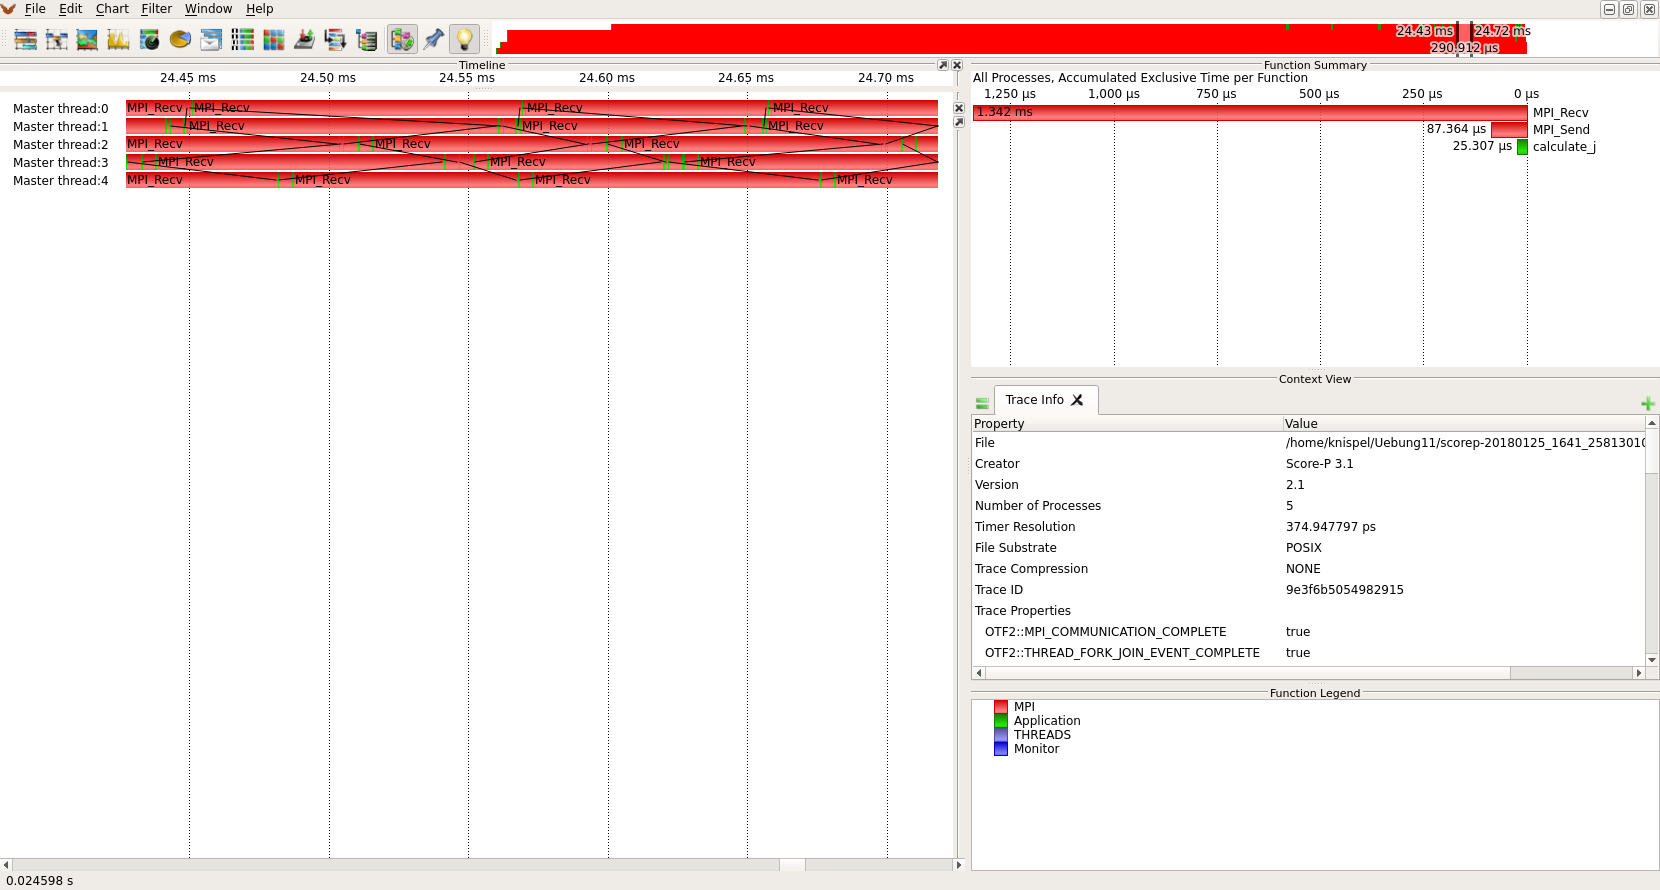
\includegraphics[width=1\textwidth]{Jacobi_2_4nodes.png} 
   \caption{Jacobi-Verfahren mit 5 Prozessoren und 4 Knoten : Phase der Synchronisation}
   \label{Jacobi_2_4nodes}
\end{figure}

\subsubsection{Phase des Einsammelns}

\begin{figure}[htbp] %  figure placement: here, top, bottom, or page
   \centering
   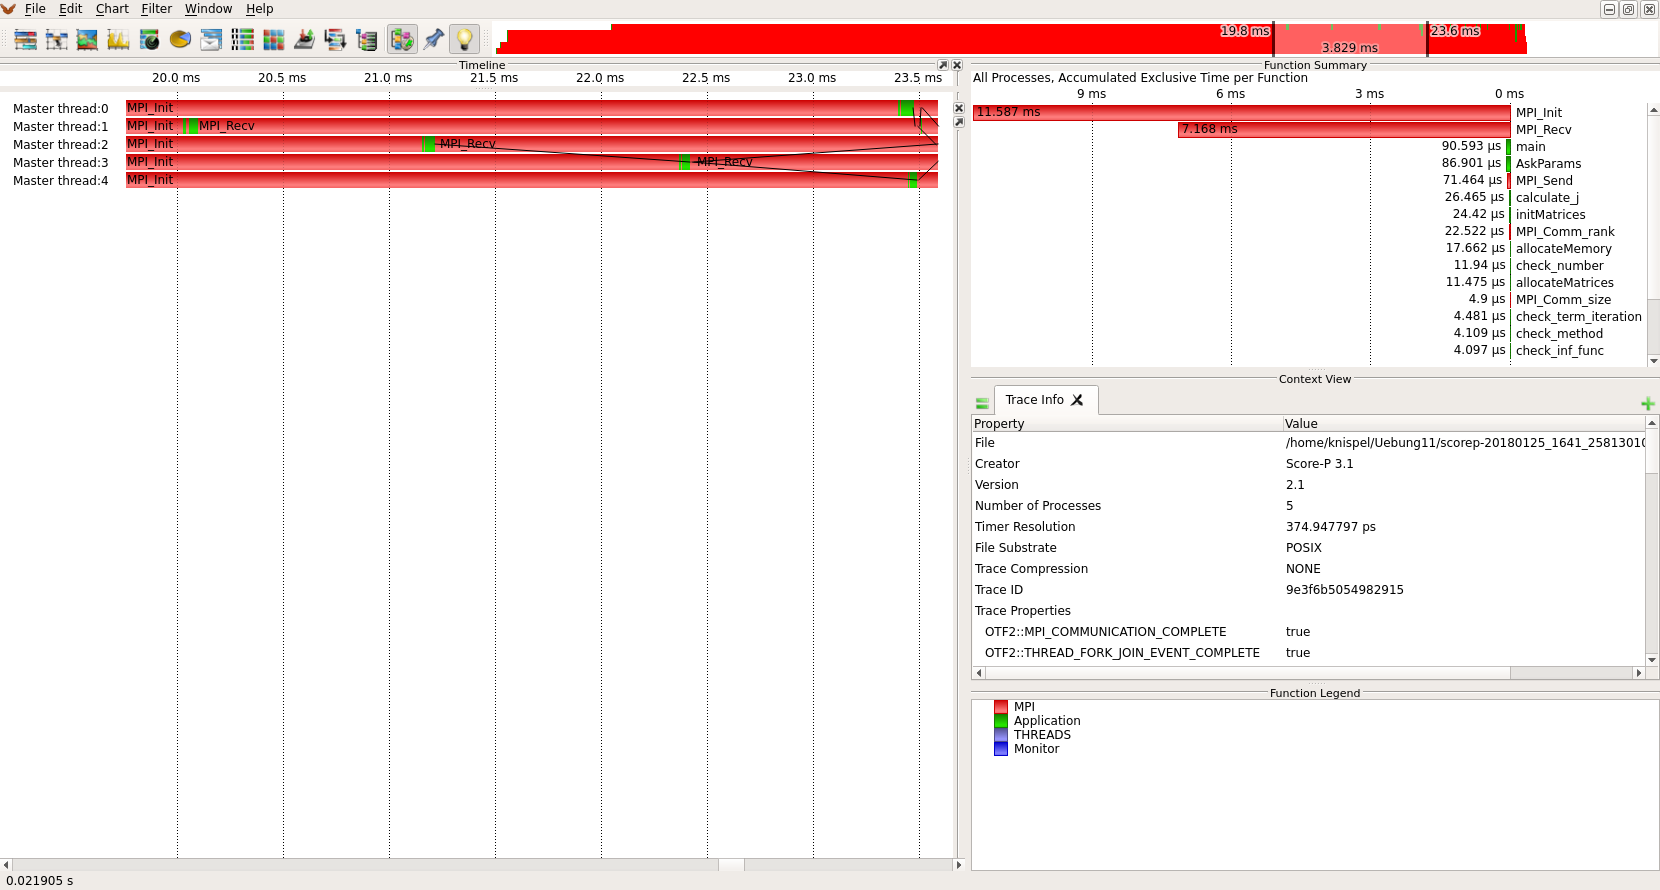
\includegraphics[width=1\textwidth]{Jacobi_1_4nodes.png} 
   \caption{Jacobi-Verfahren mit 5 Prozessoren und 4 Knoten : Phase des Einsammelns}
   \label{Jacobi_3_4nodes}
\end{figure}

\subsection{Gauß-Seidel-Verfahren}

\subsubsection{Startphase des Programms}
\begin{figure}[htbp] %  figure placement: here, top, bottom, or page
   \centering
   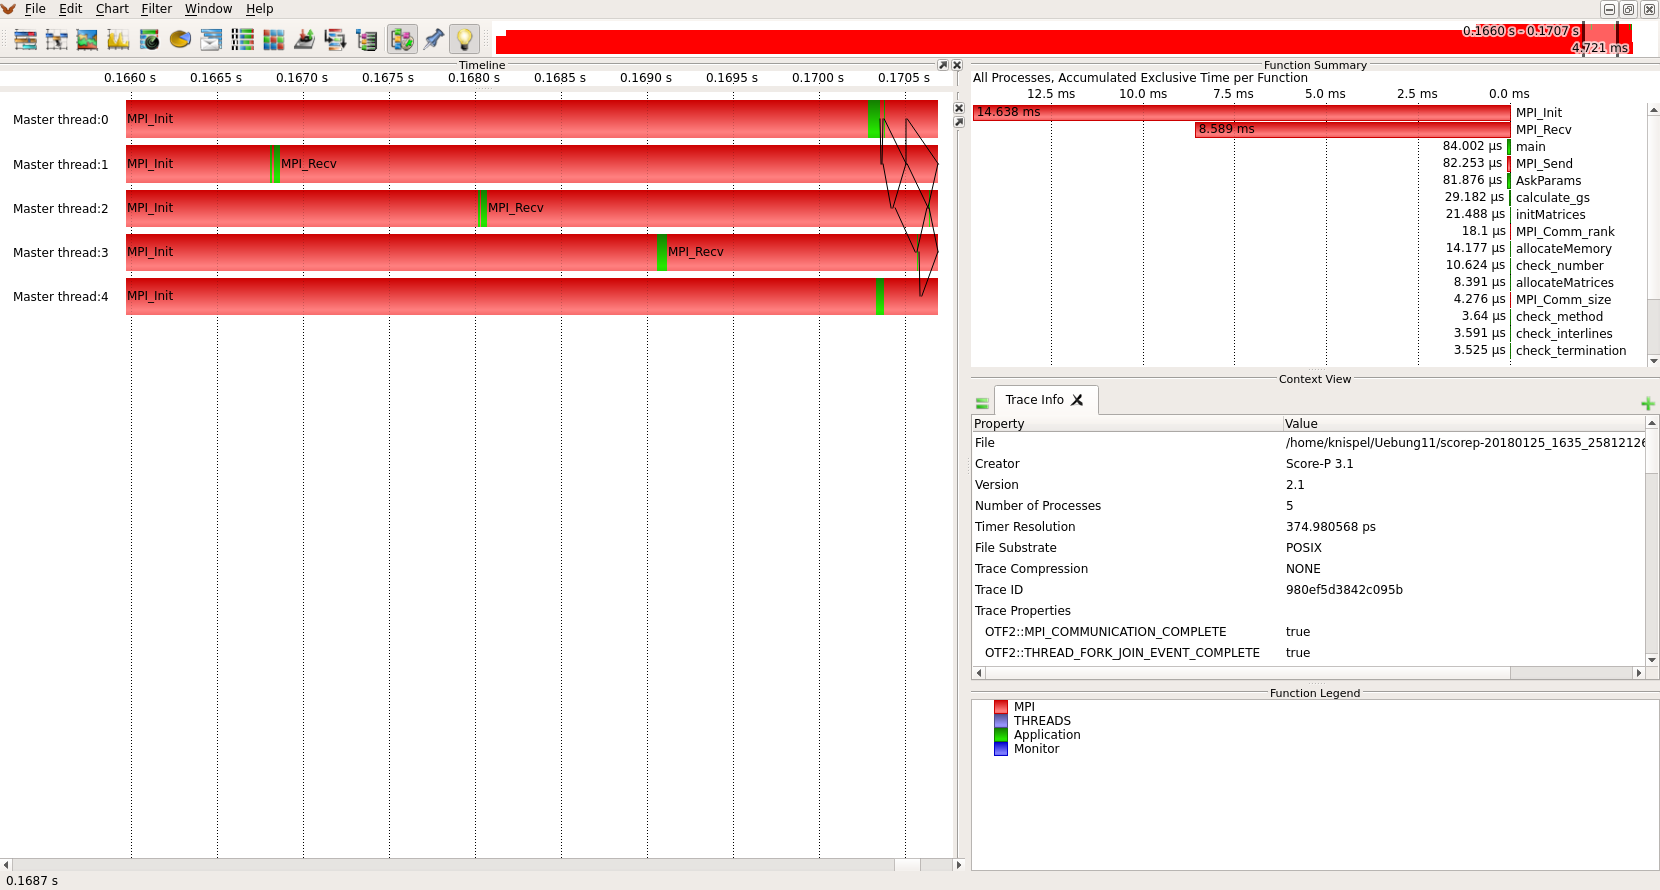
\includegraphics[width=1\textwidth]{Seidel_1_4nodes.png} 
   \caption{Gauß-Seidel-Verfahren mit 5 Prozessoren und 4 Knoten : Startphase}
   \label{Seidel_1_4nodes}
\end{figure}

\subsubsection{Phase der Synchronisation}

\begin{figure}[htbp] %  figure placement: here, top, bottom, or page
   \centering
   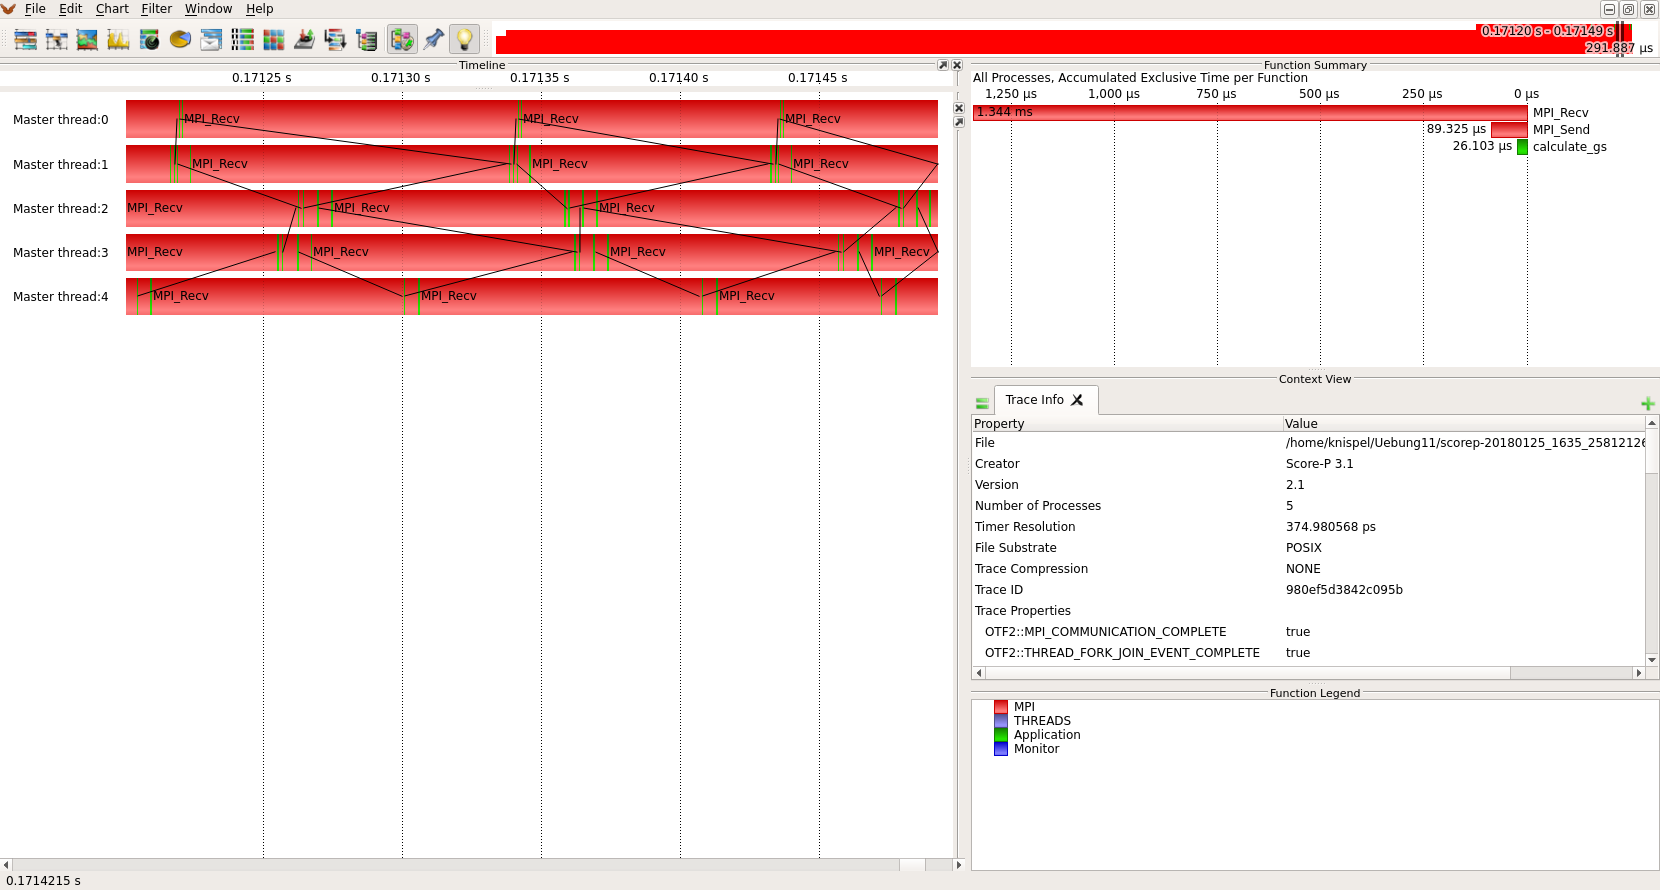
\includegraphics[width=1\textwidth]{Seidel_2_4nodes.png} 
   \caption{Gauß-Seidel-Verfahren mit 5 Prozessoren und 4 Knoten : Phase der Synchronisation}
   \label{Seidel_2_4nodes}
\end{figure}

\subsubsection{Phase des Einsammelns}

\begin{figure}[htbp] %  figure placement: here, top, bottom, or page
   \centering
   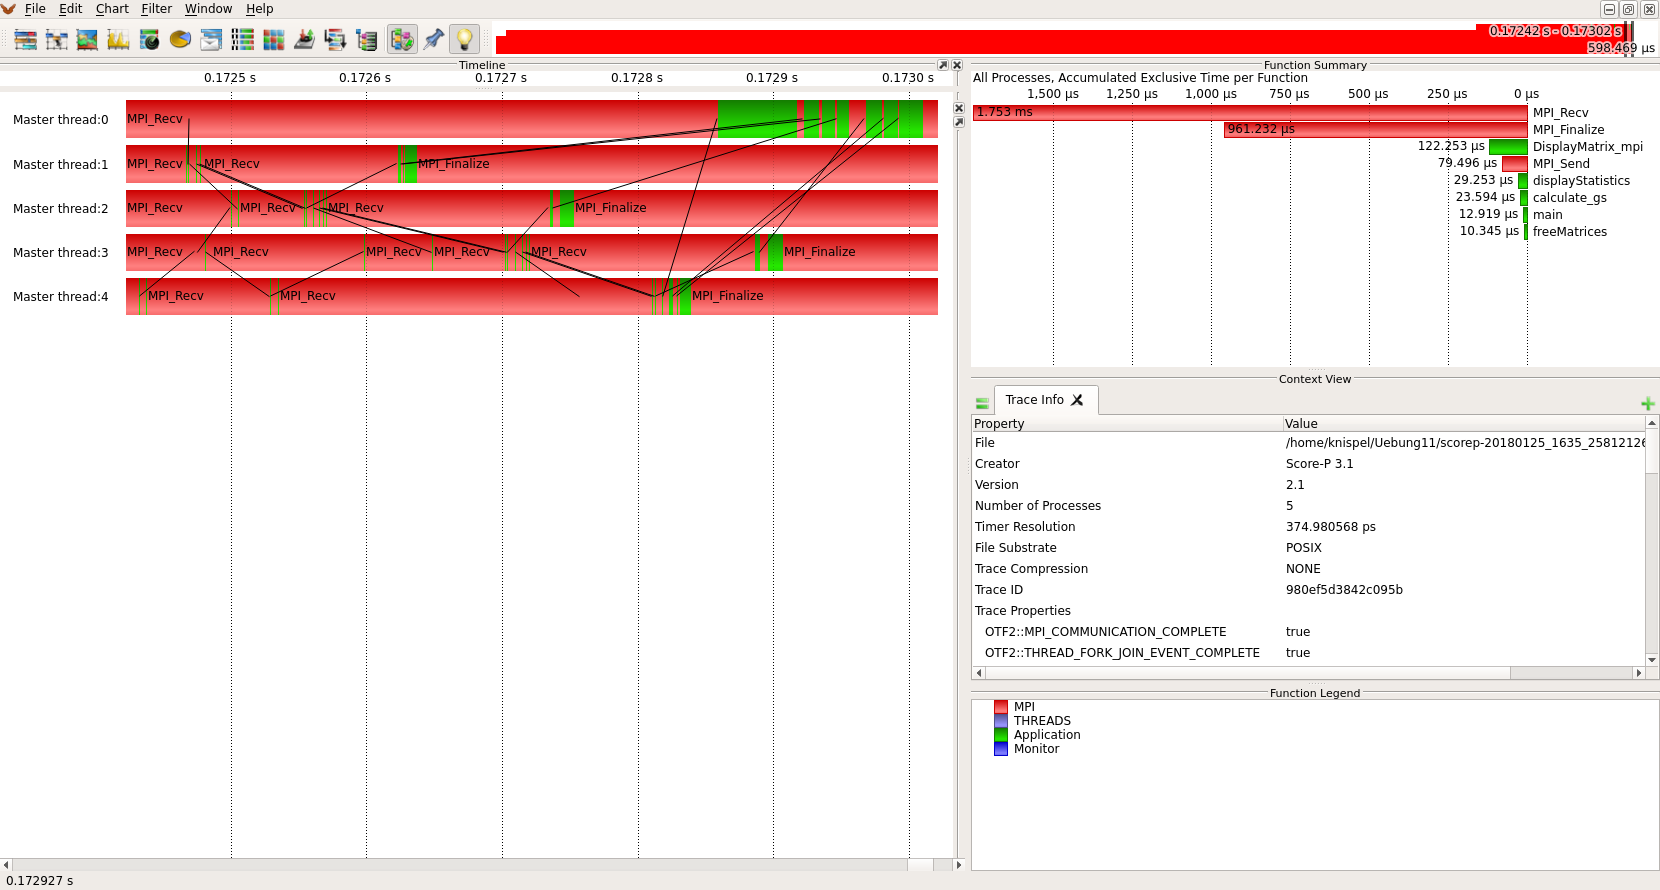
\includegraphics[width=1\textwidth]{Seidel_3_4nodes.png} 
   \caption{Gauß-Seidel-Verfahren mit 5 Prozessoren und 4 Knoten : Phase des Einsammelns}
   \label{Seidel_3_4nodes}
\end{figure}





















\end{document}